\documentclass[12pt,a4paper]{article}
\usepackage{amsmath}
\usepackage{amsfonts}
\usepackage{amssymb}
\usepackage[utf8]{inputenc}
\usepackage[T1,T2A]{fontenc}
\usepackage[english, russian]{babel}
\usepackage{graphicx}
\usepackage[left=2cm,right=2cm,top=2cm,bottom=2cm]{geometry}
\usepackage{calc}
\usepackage{wrapfig}
\usepackage{setspace}
\usepackage{indentfirst}
\usepackage{subfigure}
\usepackage[table,xcdraw]{xcolor}


\title{
Отчет о выполнении лабораторной работы 2.1.3 \\
Определение $C_p/C_\upsilon$ по скорости звука в газе
}

\author{Фокин Алексей, 922 группа}

\begin{document}
\maketitle

\paragraph{Цель работы:} 1) измерение частоты колебаний и длины волны при резонансе звуковых колебаний в газе, заполняющем трубу; 2) определение показателя адиабаты с помощью уравнения состояния идеального газа.
\paragraph{В работе используются:} звуковой генератор ГЗ; электорнный осциллограф ЭО; микрофон; телефон; раздвижная труба; теплоизолированная труба, обогреваемая водой из термостата; баллон со сжатым углекислым газом; газгольдер.

\section{Теоретическая справка}
 Один из наиболее точных методов измерения показателя адиабаты $\gamma$ основан на зависимости от него скорости распространения звуковой волны в газе. Последняя в газах определяется формулой $c = \sqrt{\frac{\gamma RT}{\mu}}$, из которой можно выразить показатель адиабаты:
 	\begin{equation}
 	\gamma = \frac{\mu}{RT}c^2,
 	\end{equation}
где $T$ --- температура газа, $\mu$ --- его молярная масса, а $R$ --- газовая постоянная. \\
Скорость $c$ звука связана с его частотой $f$ и длиной волны $\lambda$ соотношением
	\begin{equation}
	c = \lambda f.
	\end{equation}
С волнами в трубке удобнее всего работать при резонансе. Условие резонанса выглядит как
	\begin{equation}
	L = n\frac{\lambda}{2},
	\end{equation}
где $L$ --- длина трубки, $\lambda$ --- длина волны, $n$ --- целое число.\\
В данной работе при постоянной длине трубки изменяется частота звуковых колебаний $f$, а с ней и длина звуковой волны $\lambda$. Для последовательных резонансов можно записать:
	\begin{equation}
	L = n\frac{\lambda_1}{2} = (n + 1)\frac{\lambda_2}{2} = ... = (n + k)\frac{\lambda_{k + 1}}{2}
	\end{equation}
С учётом (2) имеем
	\begin{equation}
	f_{t+1} = \frac{c}{\lambda_{t+1}} = f_1 + \frac{c}{2L}t~ (t = 0, 1,..., k)
	\end{equation}
Таким образом, $c/2L$ можно найти как угловой коэффициент графика зависимости частоты от номера резонанса.
\subsection*{Экспериментальная установка}
 Схема установки, используемой в работе приведена на рис. 1.\\
	\begin{figure}[h]
		\centering
		\includegraphics[width=0.4\linewidth]{"../../../../../../Users/ПК/Desktop/Учеба/Лабы/Терма/2.1.3/установка"}
		\caption{Схема установки}
	\end{figure}
Звуковые колебания в трубе возбуждаются телефоном Т и улавливаются микрофоном М. Мембрана телефона приводится в движение переменным током звуковой частоты. В качестве источника переменной ЭДС используется звуковой генератор ГЗ. Возникающий в микрофоне сигнал возникает на экране осциллографа ЭО. \\
Микрофон и телефон присоединены к установке через тонкие резиновые трубки. Такая связь достаточна для возбуждения и обнаружения звуковых колебаний в трубе и в то же время мало возмущает эти колебания: при расчетах оба конца трубы можно считать неподвижными, а влиянием соединительных отверстий пренебречь. \\
Установка содерджит теплоизолированную трубу постоянной длины. Воздух в трубке нагревается водой из термостата.Температура газа принимается равной температуре омывающей трубу воды. 
\section{Ход работы}
	\begin{enumerate}
		\item Снимаем комнатную температуру и длину используемой трубы: $$T_\text{к} = 24,5^\circ C, L = 700~\text{мм}$$
		\item Включаем в сеть ЭО и ГЗ, даём им прогреться 5 минут. Включаем на осциллографе тумблер <<луч>> и ручками управления добиваемся прямой линии на экране. Устанавливаем нуль на звуковом генераторе.
		\item Подбираем напряжение на выходе генератора так, чтобы амплитуда колебаний при резонансе была достаточно велика. 
		\item Снимаем частоты резонансов (отмечая резонансы по резкому возрастанию амплитуды колебаний на ЭО) при разных температурах. Данные приводим в таблицах 1 и 2.
		\begin{table}[!h]
			\centering
			\begin{tabular}{|c|c|c|c|c|c|c|c|}
				\hline
				{\color[HTML]{000000} \textbf{}} & \multicolumn{7}{c|}{{\color[HTML]{000000} \textbf{Температура,$^\circ C$}}} \\ \hline
				{\color[HTML]{000000} \textbf{№ резонанса}} & {\color[HTML]{000000} \textbf{24,5}} & {\color[HTML]{000000} \textbf{30}} & {\color[HTML]{000000} \textbf{\begin{tabular}[c]{@{}c@{}}30 \\ (обратно)\end{tabular}}} & {\color[HTML]{000000} \textbf{35,4}} & {\color[HTML]{000000} \textbf{\begin{tabular}[c]{@{}c@{}}35,4\\ (обратно)\end{tabular}}} & {\color[HTML]{000000} \textbf{40}} & {\color[HTML]{000000} \textbf{\begin{tabular}[c]{@{}c@{}}40\\ (обратно\end{tabular}}} \\ \hline
				{\color[HTML]{000000} \textbf{1}} & {\color[HTML]{000000} 256} & {\color[HTML]{000000} 254} & {\color[HTML]{000000} 256} & {\color[HTML]{000000} 258} & {\color[HTML]{000000} 256} & {\color[HTML]{000000} 260} & {\color[HTML]{000000} 265} \\ \hline
				{\color[HTML]{000000} \textbf{2}} & {\color[HTML]{000000} 498,7} & {\color[HTML]{000000} 500} & {\color[HTML]{000000} 503} & {\color[HTML]{000000} 506} & {\color[HTML]{000000} 506} & {\color[HTML]{000000} 511} & {\color[HTML]{000000} 508} \\ \hline
				{\color[HTML]{000000} \textbf{3}} & {\color[HTML]{000000} 741,4} & {\color[HTML]{000000} 750} & {\color[HTML]{000000} 750} & {\color[HTML]{000000} 754} & {\color[HTML]{000000} 755} & {\color[HTML]{000000} 760} & {\color[HTML]{000000} 765} \\ \hline
				{\color[HTML]{000000} \textbf{4}} & {\color[HTML]{000000} 992} & {\color[HTML]{000000} 1000} & {\color[HTML]{000000} 1008} & {\color[HTML]{000000} 1011} & {\color[HTML]{000000} 1010} & {\color[HTML]{000000} 1016} & {\color[HTML]{000000} 1015} \\ \hline
				{\color[HTML]{000000} \textbf{5}} & {\color[HTML]{000000} 1240} & {\color[HTML]{000000} 1249} & 1251 & {\color[HTML]{000000} 1257} & {\color[HTML]{000000} 1263} & {\color[HTML]{000000} 1265} & {\color[HTML]{000000} 1265} \\ \hline
				{\color[HTML]{000000} \textbf{6}} & {\color[HTML]{000000} 1481} & 1492 & 1504 & 1520 &  &  &  \\ \hline
				\textbf{7} & 1742 &  &  &  &  &  &  \\ \hline
			\end{tabular}
		\caption{Резонансные частоты, Гц (в зависимости от температуры газа)}
		\end{table}
		\begin{table}[!h]
			\centering
			\begin{tabular}{|c|c|c|c|c|c|c|}
				\hline
				{\color[HTML]{000000} \textbf{}} & \multicolumn{6}{c|}{{\color[HTML]{000000} \textbf{Температура, $^\circ C$}}} \\ \hline
				{\color[HTML]{000000} \textbf{№ резонанса}} & {\color[HTML]{000000} \textbf{45,1}} & {\color[HTML]{000000} \textbf{\begin{tabular}[c]{@{}c@{}}45,1\\ (обратно)\end{tabular}}} & {\color[HTML]{000000} \textbf{50}} & {\color[HTML]{000000} \textbf{\begin{tabular}[c]{@{}c@{}}50\\ (обратно)\end{tabular}}} & {\color[HTML]{000000} \textbf{55}} & {\color[HTML]{000000} \textbf{\begin{tabular}[c]{@{}c@{}}55\\ (обратно)\end{tabular}}} \\ \hline
				{\color[HTML]{000000} \textbf{1}} & {\color[HTML]{000000} 262} & {\color[HTML]{000000} 261} & {\color[HTML]{000000} 263} & {\color[HTML]{000000} 265} & {\color[HTML]{000000} 269} & {\color[HTML]{000000} 267} \\ \hline
				{\color[HTML]{000000} \textbf{2}} & {\color[HTML]{000000} 514} & {\color[HTML]{000000} 515} & {\color[HTML]{000000} 517} & {\color[HTML]{000000} 520} & {\color[HTML]{000000} 523} & {\color[HTML]{000000} 523} \\ \hline
				{\color[HTML]{000000} \textbf{3}} & {\color[HTML]{000000} 764} & {\color[HTML]{000000} 765} & {\color[HTML]{000000} 771} & {\color[HTML]{000000} 770} & {\color[HTML]{000000} 780} & {\color[HTML]{000000} 777} \\ \hline
				{\color[HTML]{000000} \textbf{4}} & {\color[HTML]{000000} 1024} & {\color[HTML]{000000} 1028} & {\color[HTML]{000000} 1034} & {\color[HTML]{000000} 1031} & {\color[HTML]{000000} 1041} & {\color[HTML]{000000} 1040} \\ \hline
				{\color[HTML]{000000} \textbf{5}} & {\color[HTML]{000000} 1281} & {\color[HTML]{000000} 1281} & {\color[HTML]{000000} 1290} & {\color[HTML]{000000} 1290} & {\color[HTML]{000000} 1297} & {\color[HTML]{000000} 1300} \\ \hline
				{\color[HTML]{000000} \textbf{6}} & {\color[HTML]{000000} 1531} & {\color[HTML]{000000} } & {\color[HTML]{000000} 1540} & {\color[HTML]{000000} } & {\color[HTML]{000000} 1555} & {\color[HTML]{000000} } \\ \hline
			\end{tabular}
			\caption{Резонансные частоты, Гц (в зависимости от температуры газа)}
		\end{table}
	\item Изобразим полученные результаты на графике. По оси абсцисс откладываем номер k, а по оси ординат --- разность между частотой k+1-го резонанса и частотой первого резонанса $f_{k+1} - f_1$. (см. рис. 2) 
	\begin{figure}[!h]
		\centering
		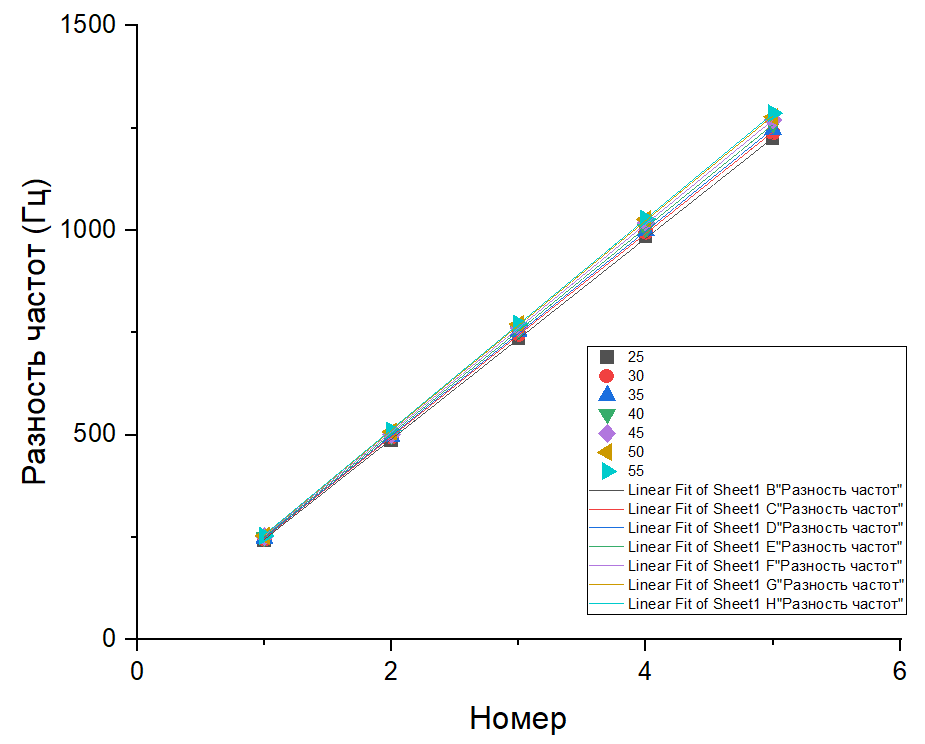
\includegraphics[width=0.8\linewidth]{../../../../../../Users/ПК/Desktop/Учеба/Лабы/Терма/2.1.3/График}
		\caption{Зависимость разности k+1-й и первой частот от номера резонанса k}
		\label{fig:}
	\end{figure}
	\item Получаем коэффициенты наклона, равные c/2L (табл. 3)
	\begin{table}[!h]
		\centering
		\begin{tabular}{|l|l|l|l|l|l|l|l|}
			\hline
			\textbf{Температура, $^\circ C$} & {\color[HTML]{000000} 25} & {\color[HTML]{000000} 30} & {\color[HTML]{000000} 35} & {\color[HTML]{000000} 40} & {\color[HTML]{000000} 45} & {\color[HTML]{000000} 50} & {\color[HTML]{000000} 55} \\ \hline
			\textbf{с/2L} & {\color[HTML]{000000} 245,1$\pm$0,4} & {\color[HTML]{000000} 248,1$\pm$0,3} & {\color[HTML]{000000} 249,5$\pm$0,4} & {\color[HTML]{000000} 251,6$\pm$0,3} & {\color[HTML]{000000} 253,9$\pm$0,5} & {\color[HTML]{000000} 256,0$\pm$0,5} & {\color[HTML]{000000} 257,0$\pm$0,3} \\ \hline
		\end{tabular}
	\caption{Коэффициенты наклона графиков, с$^{-1}$ (в зависимости от температуры газа)}
	\end{table}
	\item Для каждого значения температуры вычисляем $\gamma$ по формуле (1).
		\begin{table}[!h]
			\centering
			\begin{tabular}{|l|l|l|l|l|l|l|l|}
				\hline
				\textbf{Температура, $^\circ C$} & {\color[HTML]{000000} 25} & {\color[HTML]{000000} 30} & {\color[HTML]{000000} 35} & {\color[HTML]{000000} 40} & {\color[HTML]{000000} 45} & {\color[HTML]{000000} 50} & {\color[HTML]{000000} 55} \\ \hline
				\textbf{$\gamma$} & {\color[HTML]{000000} 1,38118} & {\color[HTML]{000000} 1,38951} & {\color[HTML]{000000} 1,38063} & {\color[HTML]{000000} 1,38334} & {\color[HTML]{000000} 1,3866} & {\color[HTML]{000000} 1,3878} & {\color[HTML]{000000} 1,37735} \\ \hline
			\end{tabular}
		\end{table}
	Погрешность также оцениваем из ф-лы (1), она получается равной $\varepsilon = 10^{-4}$.
	\item Таким образом, среднее значение показателя адиабаты получаем равным $$\gamma = 1,3837\pm0,0001$$
	\end{enumerate}
\section{Выводы}
	\begin{enumerate}
		\item В ходе данной работы была проверена предложенная экспериментальная методика.
		\item С высокой точностью был измерен показатель адиабаты воздуха.
		\item Была проверена зависимость скорости звука в газе от температуры.
	\end{enumerate}
\end{document}
